\documentclass[border=3pt]{standalone}

\usepackage{amssymb}
\usepackage{amsfonts}
\usepackage{mathrsfs}
\usepackage{amsthm}
\usepackage{amsmath}
\usepackage{xcolor}
\usepackage{hyperref}
\usepackage{libertinus}
\usepackage{dsfont}
\usepackage{bm}
\usepackage{enumitem}
\usepackage{caption}
\usepackage{subcaption}
\usepackage{tikz}
\usepackage{quiver}

\newcommand{\R}{\mathbb{R}}
\newcommand{\C}{\mathbb{C}}
\newcommand{\N}{\mathbb{N}}
\newcommand{\Z}{\mathbb{Z}}
\newcommand{\Q}{\mathbb{Q}}

% differentials and derivatives
\renewcommand{\d}{\mathrm{d}}
\newcommand{\dd}{\,\d}
\newcommand{\pddf}[2]{\frac{\partial#1}{\partial#2}}
\newcommand{\ddt}{\frac{\d }{\d t}}
\newcommand{\ddtz}{\left.\ddt\right|_{t=0}}
\usepackage{tikz}
\usetikzlibrary{braids}

\tikzcdset{every arrow/.append style={no head,line width=0.45pt}}

\begin{document}
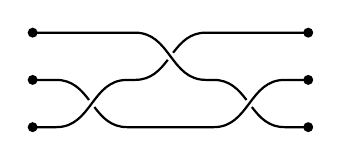
\begin{tikzpicture}
   % Named braid, rotated so it runs left-to-right
   \pic[
   rotate=90,
   name=b,
   braid/.cd,
   number of strands=3,
   width=6mm, % smaller than the default spacing
   every strand/.style={thick},
   ] {braid={s_1 s_2^{-1} s_1}};

   % dots on the left side (starts)
   \foreach \i in {1,2,3}
   \fill (b-\i-s) circle (1.8pt);

   % dots on the right side (ends)
   \foreach \i in {1,2,3}
   \fill (b-\i-e) circle (1.8pt);
\end{tikzpicture}
\end{document}